%%%%%%%%%%%%%%%%%%%%%%%%%%%%%%%%%%%%%%%%%%%%%%%%%%%%%%%%%%%%%%%%%%%%%
%% Please do not use \input{...} to include other tex files.       %%
%% Submit your LaTeX manuscript as one .tex document.              %%
% Note (ET): We will do this at the end!
%%                                                                 %%
%% All additional figures and files should be attached             %%
%% separately and not embedded in the \TeX\ document itself.       %%
% TODO: discuss this! might mean we have to generate all figures externaly
%%%%%%%%%%%%%%%%%%%%%%%%%%%%%%%%%%%%%%%%%%%%%%%%%%%%%%%%%%%%%%%%%%%%%
% some aditional \documentclass options:
% \documentclass[referee,...]{sn-jnl}% referee option is meant for double line spacing
%\documentclass[lineno,...]{sn-jnl}% to print line numbers in the margin use lineno option
\RequirePackage{tikz}
\documentclass[pdflatex,sn-basic]{template/sn-jnl}% Basic Springer Nature Reference Style/Chemistry Reference Style
%%\documentclass[sn-mathphys]{sn-jnl}% Math and Physical Sciences Reference Style
%%\documentclass[sn-aps]{sn-jnl}% American Physical Society (APS) Reference Style
%%\documentclass[sn-vancouver]{sn-jnl}% Vancouver Reference Style
%%\documentclass[sn-apa]{sn-jnl}% APA Reference Style
%%\documentclass[sn-standardnature]{sn-jnl}% Standard Nature Portfolio Reference Style
%%\documentclass[default]{sn-jnl}% Default
%%\documentclass[default,iicol]{sn-jnl}% Default with double column layout


%%%% Standard Packages
%%<additional latex packages if required can be included here>
%%%%%%%%%%%%%%%%%%%%%%%%%%%%%%%%%%%%%%%%%%%%%%%%%%%
%% definitions of variables
%%%%%%%%%%%%%%%%%%%%%%%%%%%%%%%%%%%%%%%%%%%%%%%%%
% general symbols
%%%%%%%%%%%%%%%%%%%%%%%%%%%%%%%%%%%%%%%%%%%%%%%%%
\DeclareMathOperator{\tr}{tr}
\newcommand{\bA}{\boldsymbol{A}}
\newcommand{\bI}{\boldsymbol{I}}
\newcommand{\bL}{\boldsymbol{L}}
\newcommand{\bvarepsilon}{\boldsymbol{\varepsilon}}
\newcommand{\bsigma}{\boldsymbol{\sigma}}
\newcommand{\TP}{^\text{T}}
%%%%%%%%%%%%%%%%%%%%%%%%%%%%%%%%%%%%%%%%%%%%%%%%%
% homogenization vars
%%%%%%%%%%%%%%%%%%%%%%%%%%%%%%%%%%%%%%%%%%%%%%%%%
\newcommand{\eMod}{E}  % youngs modulus
\newcommand{\eModEff}{\eMod_{\text{eff}}}  % mocroscopic youngs modulus
\newcommand{\poission}{\nu}  % poissionsratio
\newcommand{\poissionZero}{\poission^{(0)}}  % poissionsratio
\newcommand{\poissionEff}{\poission_{\text{eff}}}  % poissionsratio effective
\newcommand{\fc}{f_{\text{c}}}  % compressive strength
\newcommand{\fcInf}{{\fc}_\infty}  % compressive strength
\newcommand{\ft}{f_{\text{t}}}  % tensile strength
\newcommand{\ftInf}{{\ft}_\infty}  % compressive strength
\newcommand{\fcEff}{{\fc}_{,\text{eff}}}  % compressive strength
\newcommand{\body}{\Omega}  % body
\newcommand{\phaseIndex}{r}  % index letter for different phases
\newcommand{\matrixIndex}{\text{m}}  % index letter for different phases
\newcommand{\inclIndex}{\text{i}}  % index letter for different phases
\newcommand{\bodyPhase}{\body^{(\phaseIndex)}}
\newcommand{\volFrac}{c}
\newcommand{\volFracPhase}{\volFrac^{(\phaseIndex)}}
\newcommand{\volFracMatrix}{\volFrac^{(\matrixIndex)}}
\newcommand{\volFracIncl}{\volFrac^{(\inclIndex)}}
\newcommand{\volFracZero}{\volFrac^{(0)}}
\newcommand{\radius}{R}
\newcommand{\radiusPhase}{\radius^{(\phaseIndex)}}
\newcommand{\bulkMod}{K}
\newcommand{\bulkModPhase}{\bulkMod^{(\phaseIndex)}}
\newcommand{\bulkModMatrix}{\bulkMod^{(\matrixIndex)}}
\newcommand{\bulkModIncl}{\bulkMod^{(\inclIndex)}}
\newcommand{\bulkModZero}{\bulkMod^{(0)}}
\newcommand{\bulkModEff}{\bulkMod_{\text{eff}}}
\newcommand{\shearMod}{G}
\newcommand{\shearModPhase}{\shearMod^{(\phaseIndex)}}
\newcommand{\shearModMatrix}{\shearMod^{(\matrixIndex)}}
\newcommand{\shearModIncl}{\shearMod^{(\inclIndex)}}
\newcommand{\shearModZero}{\shearMod^{(0)}}
\newcommand{\shearModEff}{\shearMod_{\text{eff}}}
\newcommand{\matStiff}{\bL}
\newcommand{\matStiffZero}{\matStiff^{(0)}}
\newcommand{\matStiffPhase}{\matStiff^{(\phaseIndex)}}
\newcommand{\matStiffEff}{\matStiff_{\text{eff}}}
\newcommand{\orthProjV}{\bI_{\text{V}}}
\newcommand{\orthProjD}{\bI_{\text{D}}}
\newcommand{\strain}{\bvarepsilon}
\newcommand{\strainPhase}{\strain^{(\phaseIndex)}}
\newcommand{\strainZero}{\strain^{(0)}}
\newcommand{\stress}{\bsigma}
\newcommand{\stressZero}{\stress^{(0)}}
\newcommand{\stressMatrix}{\stress^{(\matrixIndex)}}
\newcommand{\stressD}{\stress_{\text{D}}}
\newcommand{\stressTest}{\stress^{\text{test}}}
\newcommand{\concentration}{\bA}
\newcommand{\concentrationPhase}{\concentration^{(\phaseIndex)}}
\newcommand{\concentrationZero}{\concentration^{(0)}}
\newcommand{\dilConcentration}{\concentration_{\text{dil}}}
\newcommand{\dilConcentrationPhase}{\dilConcentration^{(\phaseIndex)}}
\newcommand{\dilConcentrationIncl}{\dilConcentration^{(\inclIndex)}}
\newcommand{\dilConcentrationVPhase}{A^{(\phaseIndex)}_{\text{dil,V}}}
\newcommand{\dilConcentrationDPhase}{A^{(\phaseIndex)}_{\text{dil,D}}}
\newcommand{\dilConcentrationVIncl}{A^{(\inclIndex)}_{\text{dil,V}}}
\newcommand{\dilConcentrationDIncl}{A^{(\inclIndex)}_{\text{dil,D}}}
\newcommand{\auxAlphaZero}{\alpha^{(0)}}
\newcommand{\auxBetaZero}{\beta^{(0)}}
\newcommand{\Jtwo}{J_2}
\newcommand{\JtwoTest}{\Jtwo^{\text{test}}}
\newcommand{\JtwoZero}{\Jtwo^{(0)}}
\newcommand{\JtwoMatrix}{\Jtwo^{(\matrixIndex)}}
\newcommand{\force}{f} 
\newcommand{\forceTest}{\force^{\text{test}}} 
\newcommand{\thermCond}{\chi}
\newcommand{\thermCondZero}{\thermCond^{(0)}}
\newcommand{\thermCondPhase}{\thermCond^{(\phaseIndex)}}
\newcommand{\thermCondMatrix}{\thermCond^{(\matrixIndex)}}
\newcommand{\thermCondIncl}{\thermCond^{(\inclIndex)}}
\newcommand{\thermCondHom}{\thermCond_{\text{eff}}}
\newcommand{\concentrationThermCondPhase}{A_{\chi}^{(\phaseIndex)}}
\newcommand{\concentrationThermCondIncl}{A_{\chi}^{(\inclIndex)}}
\newcommand{\Ivol}{\bI_{\text{V}}}
\newcommand{\Idev}{\bI_{\text{D}}}
%%%%%%%%%%%%%%%%%%%%%%%%%%%%%%%%%%%%%%%%%%%%%%%%%
% fem model vars
%%%%%%%%%%%%%%%%%%%%%%%%%%%%%%%%%%%%%%%%%%%%%%%%%
\newcommand{\currentn}{n+1}
\newcommand{\lastn}{n}
\newcommand{\DOH}{\alpha} % degree of hydration
\newcommand{\DOHLast}{\DOH^{\lastn}} % degree of hydration of last timestep
\newcommand{\DOHCurrent}{\DOH^{\currentn}} % degree of hydration of last timestep
\newcommand{\DOHmax}{\alpha_{\text{max}}} % degree of hydration
\newcommand{\DOHt}{\alpha_{\text{t}}} % degree of hydration
\newcommand{\DOHZero}{\alpha_{0}} % degree of hydration
\newcommand{\heat}{Q} % cummulative heat release
\newcommand{\heatInf}{Q_{\infty}} % total cummulative heat release
\newcommand{\zeit}{t} % time
\newcommand{\temp}{T} % time
\newcommand{\tempCurrent}{\temp^{\currentn}} % time n+1
\newcommand{\tempLast}{\temp^{\lastn}} % time n
\newcommand{\tempRef}{\temp_{\text{ref}}}
\newcommand{\dTdt}{\frac{\partial \temp}{\partial \zeit}}  % time derivative of temperature
\newcommand{\dQdt}{\frac{\partial \heat}{\partial \zeit}}  % time derivative of heat
\newcommand{\heatCapSpecific}{C} % specific heat capacity
\newcommand{\density}{\rho} % density
\newcommand{\thermCondEff}{\lambda} % effective thermal conductivity %%% \thermCond
\newcommand{\dDOHdt}{\frac{\partial \DOH}{\partial \zeit}}  % time derivative of DoH
\newcommand{\affinity}{A} % temperature \affinityTempscaled affinity
\newcommand{\affinityTemp}{\tilde{\affinity}} % temperature \affinityTempscaled affinity
\newcommand{\affinityScale}{a} % scale factor for affinity
\newcommand{\hydParBone}{B_1}
\newcommand{\hydParBtwo}{B_2}
\newcommand{\hydParEta}{\eta}
\newcommand{\function}{f}
\newcommand{\strengthX}{X}
\newcommand{\strengthXInf}{\strengthX_\infty}
\newcommand{\strengthExp}{a}
\newcommand{\strengthXExp}{\strengthExp_\strengthX}
\newcommand{\strengthCExp}{\strengthExp_{\fc}}
\newcommand{\strengthTExp}{\strengthExp_{\ft}}
\newcommand{\stiffExp}{\strengthExp_{\eMod}}
\newcommand{\eModInf}{\eMod_\infty}  % youngs modulus
\newcommand{\activE}{E_{\text{a}}}
\newcommand{\gasConst}{R}
\newcommand{\wc}{r_{\text{wc}}}
%%%%%%%%%%%%%%%%%%%%%%%%%%%%%%%%%%%%%%%%%%%%%%%%%
% beam design vars
%%%%%%%%%%%%%%%%%%%%%%%%%%%%%%%%%%%%%%%%%%%%%%%%%
\newcommand{\beamLength}{l}
\newcommand{\beamDistrLoad}{q}
\newcommand{\beamPointLoad}{F}
\newcommand{\beamMaxMoment}{M_{\text{max}}}
\newcommand{\beamMaxShearForce}{F_{\tau,\text{max}}}
\newcommand{\beamHeight}{h}
\newcommand{\beamHeightEff}{\beamHeight_{\text{eff}}}
\newcommand{\beamCover}{c}
\newcommand{\beamSteelDiameter}{d_{\text{st}}}
\newcommand{\beamConcreteSF}{\gamma_{\text{c}}}
\newcommand{\beamSteelSF}{\gamma_{\text{s}}}
\newcommand{\beamTimeSF}{\alpha_{\text{cc}}}
\newcommand{\beamfcd}{f_{\text{cd}}}
\newcommand{\beamfsd}{f_{\text{ywd}}}
\newcommand{\beamfs}{f_{\text{yk}}}





  % tex commands not variable
\newcommand{\workflowGraph}{paper_workflow_graph.gv.pdf}
\newcommand{\snakemakeGraph}{snakemake_optimization_graph.pdf}
   % tex commands created by script

\newcommand{\figures}{../figures/} % scale factor for affinity
%%%%

%%%%%=============================================================================%%%%
%%%%  Remarks: This template is provided to aid authors with the preparation
%%%%  of original research articles intended for submission to journals published 
%%%%  by Springer Nature. The guidance has been prepared in partnership with 
%%%%  production teams to conform to Springer Nature technical requirements. 
%%%%  Editorial and presentation requirements differ among journal portfolios and 
%%%%  research disciplines. You may find sections in this template are irrelevant 
%%%%  to your work and are empowered to omit any such section if allowed by the 
%%%%  journal you intend to submit to. The submission guidelines and policies 
%%%%  of the journal take precedence. A detailed User Manual is available in the 
%%%%  template package for technical guidance.
%%%%%=============================================================================%%%%

\jyear{2022}%


\raggedbottom
%%\unnumbered% uncomment this for unnumbered level heads

\begin{document}

\title[Awesome Article Title]{Awesome Article Title}

%%=============================================================%%
%% Prefix	-> \pfx{Dr}
%% GivenName	-> \fnm{Joergen W.}
%% Particle	-> \spfx{van der} -> surname prefix
%% FamilyName	-> \sur{Ploeg}
%% Suffix	-> \sfx{IV}
%% NatureName	-> \tanm{Poet Laureate} -> Title after name
%% Degrees	-> \dgr{MSc, PhD}
%% \author*[1,2]{\pfx{Dr} \fnm{Joergen W.} \spfx{van der} \sur{Ploeg} \sfx{IV} \tanm{Poet Laureate} 
%%                 \dgr{MSc, PhD}}\email{iauthor@gmail.com}
%%=============================================================%%
% TODO: discuss order of authors, do we need to include more?


\author*[1]{\fnm{Atul} \sur{Agrawal}}\email{atul.agrawal@tum.de}
\equalcont{These authors contributed equally to this work.}

\author[2]{\fnm{Erik} \sur{Tamsen}}\email{erik.tamsen@bam.de}
\equalcont{These authors contributed equally to this work.}

\author[1]{\fnm{Faidon-Stelios} \sur{Koutsourelakis}}\email{p.s.koutsourelakis@tum.de}

\author[2]{\fnm{Jörg F.} \sur{Unger}}\email{joerg.unger@bam.de}

\affil*[1]{\orgdiv{Data-driven Materials Modeling}, \orgname{Technische Universität München}, \orgaddress{\street{Boltzmannstraße 15}, \city{Garching}, \postcode{85748}, \country{Germany}}}

\affil[2]{\orgdiv{Modeling and Simulation}, \orgname{Bundesanstalt für Materialforschung und -prüfung}, \orgaddress{\street{Unter den Eichen 87}, \city{Berlin}, \postcode{12205}, \country{Germany}}}


%%==================================%%
%% sample for unstructured abstract %%
%%==================================%%
\abstract{Amazing introduction to this topic, talking about problems with local optimization on mix and structre.
We are ...
By applying .... stochastic methods, the quality of the data can be estimated.
Automated workflow to simplify addition of additional data points and general reproducibility.}

\keywords{performance oriented design, stochastic optimization, precast concrete, mix design}

%%\pacs[JEL Classification]{D8, H51}

%%\pacs[MSC Classification]{35A01, 65L10, 65L12, 65L20, 65L70}

\maketitle


\section{Introduction}\label{sec:introduction}
Precast concrete elements play a critical role in achieving efficient, low cost and sustainable structures.
The controlled production environment allows for higher quality products and enables the mass production of elements.
In the standard design approach, engineers or architects select a structure, estimate the loads, choose mechanical properties, and design the element accordingly. 
If the results are not satisfactory, the required mechanical properties are iteratively adjusted, aiming to improve the design.
This approach is fine, when the choice of mixtures is limited and the expected concrete properties are well known.
There are various published methods to automate this process and optimize the beam design at this level.
Computer aided beam design optimization dates back at least 50 year, e.g. \cite{Haung1967}.
Generally the objective is reducing costs, with the design variables being the beam geometry, the amount and location of the reinforcement and sometimes the compressive strength of the concrete \cite{Chakrabarty_1992, Coello_1997, Pierott_2021, Shobeiri_2023} .
Most publications focus on analytical functions based on norms and well known rules of thumb.
In recent years the use of alternative binders in the concrete mix design has increased, mainly to reduce the environmental impact and cost of concrete but also to improve and modify specific properties.
This is a challenge as the concrete mix is no longer a constant and is itself subjected to optimization.
Known heuristics might no longer apply to the new materials and old design approaches might fail to produce optimal results.
In addition it is not favorable to choose from a predetermined set of possible mixes, as this would either lead to an exaggerated number of required experiments or a limiting subset of the possible design space.
There exist literature studying the optimization of specific concrete properties on the concrete mix \cite{Lisienkova_2021, Kondapally_2022}.
\begin{figure}[b]%
	\centering
	\includegraphics[width=1.0\textwidth]{../figures/\designStandard}
	\caption{Classical design approach, where the required material properties are defined before the mix is defined.}\label{fig:standard_design}
\end{figure}
The objective in that literature is normally to either improve some mechanical property like durability within constraints, or to minimize e.g. the amount of concrete while keeping other properties above a threshold.
When designing elements subjected to various requirements, both on the material and structural level, including workability of the fresh concrete, durability of the structure, maximum acceptable temperature, minimal cost and global warming potential, the optimal solution is not apparent and will change depending on each individual project.
The conventional method of design does not allow for an concurrent optimization of structural measures and concrete mix composition, as the structural  design and the concrete mix design are inversely coupled, c.f. Figure \ref{fig:standard_design}.
The lack of coordination between the designer and the concrete manufacturer can therefore lead to suboptimal solutions, as neither party possesses all the relevant information.
A first step to address these limitations is the incorporation of compressive strength during a optimization in the beam design phase.
Higher compressive strength usually correlates with lager amount of cement and therefore higher cost as well as global warming potential.
This approach has shown promising results in achieving improved structural efficiency while considering environmental impact \cite{dos_Santos_2023}.
To be able to find a part specific optimum, individual data of the manufacturer and specific mix options must be integrated.
Therefore, there is still a need for a comprehensive optimization procedure that can seamlessly integrate concrete mixture optimization and structural simulations, ensuring structurally sound and buildable elements with minimized environmental impact for part specific data.
\\
\begin{figure}[b]%
	\centering
	\includegraphics[width=1.0\textwidth]{../figures/\designProposed}
	\caption{Presented design approach that allows for a holistic optimization.}\label{fig:proposed_workflow}
\end{figure}
%%%%%%%%%%%%%%%%%%%%
In this paper, we present a holistic optimization procedure that combines concrete mixture optimization with the structural response of precast concrete elements, using structural simulations as constraints to ensure structural integrity, limit the maximum temperature and ensure an adequate time of demolding.
This inverts the classical design pipeline.
As a first step the concrete mix is defined.
Based on the output, the beam design is created, c.f. Figure \ref{fig:proposed_workflow}.
The chosen example of this optimization procedure is to reduce the GWP of precast concrete elements. 
By integrating the concrete mixture optimization and structural design processes, engineers can tailor the concrete properties to meet specific requirements of the customer and manufacturer.
This approach opens up possibilities for performance prediction and optimization for new mixture that fall outside the standard range of well-known concrete.
To the best of our knowledge there are no published works that combine the material and structural level in one flexible optimization framework.
In addition to changing the order of the design steps, the proposed framework allows to directly integrate experimental data and propagate the identified uncertainties.
This allows a straight forward integration of new data and and quantification of uncertainties regarding the predictions.
The proposed framework consists of three main parts.
First, an automated and reproducible parameter identification method to calibrate the models.
Second, a gradient-based optimization method for non-differentiable functions, including constraints.
Third, a flexible workflow combining the models and functions required for the respective problem. 
For this publication a well known example of a simply supported, reinforced, rectangular beam  has been chosen.
The design problem was originally published in \cite{everard1966reinforced}.
It has been used to showcase different optimization schemes, e.g. \cite{Chakrabarty_1992}, \cite{Coello_1997}, \cite{Pierott_2021}.
The experimental data used in the parameter identification step is mainly sourced from \cite{gruyaert2011}.
The objective is to reduce the overall global warming potential of the part.
This objective is a particularly meaningful as the cement industry, a major contributor to GWP, accounts for approximately 8\% of the total anthropogenic GWP. 
Reducing the environmental impact of cement production becomes crucial in the pursuit of sustainable construction practices.
In addition, the reduction of cement is also correlated to the reduction of cost, as cement is generally the most expensive component of the concrete mix \cite{Paya_Zaforteza_2009}.
There are three direct ways to reduce the amount of cement.
First, replace the cement with a substitute with a lower carbon footprint.
This can change mechanical properties, but does not necessarily mean a reduction in strength.
Second, increase the amount of aggregates.
This also changes effective properties and needs to be balanced with the workability and the limits due to the applications.
Third, decrease the overall volume of concrete.
In addition, when analyzing the whole life-cycle of concrete, both cost and GWP can be reduced by increasing the durability and therefore extending the lifetime of the object.
To showcase the methods capability, two design variables have been chosen, the height of the beam and the ratio of ordinary Portland cement (OPC) to its replacement binder ground granulated blast furnace slack, a by-product of iron industry.\\
%
The value of this manuscript lies in two main contributions. 
Firstly, it presents the possibility to automatically compute relevant Key Performance Indicators (KPIs) at the structural level, based on input values that incorporate parameters relevant to the concrete mix design, inverting the classical design pipeline.
This allows for a comprehensive evaluation of both structural performance and environmental impact. 
Secondly, the paper details the numerical methods employed to conduct a robust optimization process without derivatives, taking into account uncertainties based on raw experimental data.
\\
% this might change and needs to be adapted
The paper starts  with the theoretical background of the parameter identification method in Section \ref{sec:calibration}.
It is followed by the optimization method in Section \ref{sec:optimization} and some numerical experiments showcasing the method in \ref{sec:numericalexperiments}.
Section \ref{sec:data} gives details on the example problem and an overview of the available experimental data.
The following Section \ref{sec:models} gives an overview of the material models and applied assumption. 
In Section \ref{sec:results} all parts, the experimental data, the calibration method, the numerical models and the optimization framework are combined to demonstrate the effectiveness and practicality of the proposed approach.
The publication finishes with a conclusion and outlook in Section \ref{sec:conclusion}.

\section{Models}\label{sec:models}

\subsection{Notes on Early Age Concrete Model}
Plan is do collect notes, information on the early age concrete model I am implementing.
Currently the plan is to include temperature and humidity and couple them the respective mechanical fields.
I will start with the temperature field.

\subsection{Modeling of the temperature field}
Temperature is generally described as

\begin{align}
	\rho C\frac{\partial T}{\partial t} = \nabla \cdot (\lambda \nabla T) + \frac{\partial Q}{\partial t} \label{eq:heat1}
\end{align}
$\lambda$ is the effective thermal conductivity in Wm$^{-1}$K$^{-1}$.
$C$ is the specific heat capacity.
$\rho$ is the density.
$\rho C$ is the volumetric heat capacity in Jm$^{-3}$K$^{-1}$.
$Q$ is the volumetric heat, due to hydration, it is also called the latent heat of hydration, or the heat source in Jm$^{-3}$.
For now we assume the density, the thermal conductivity and the volumetric heat capacity as constant, however there are models that make them dependent on the temperature, moisture and/or the hydration.


\subsubsection{Degree of hydration $\alpha$}
The degree of hydration $\alpha$ is defined as the ratio between the cumulative heat $Q$ at time $t$ and the total theoretical volumetric heat by complete hydration $Q_{\infty}$,
\begin{align}
	\alpha(t) = \frac{Q(t)}{Q_{\infty}},
\end{align}
by assuming a linear relation between the degree of hydration and the heat development.
Therefore the time derivative of the heat source $\dot{Q}$ can be rewritten in terms of $\alpha$, 
\begin{align}
	\frac{\partial Q}{\partial t} = \frac{\partial \alpha}{\partial t} Q_{\infty}. \label{eq:qdotalphadot}
\end{align}
There are formulas to approximate total potential heat based on composition, approximated values range between 300 and 600 J/g of binder for different cement types, e.g. Ordinary Portland cement $Q_{\infty} =$ 375–525 or Pozzolanic cement $Q_{\infty} =$ 315–420.  

\subsubsection{Affinity}
The heat release can be modeled based on the chemical affinity $A$ of the binder.
The hydration kinetics can be defined as a function of affinity at a reference temperature $\tilde{A}$ and a temperature dependent scale factor ${a}$
\begin{align}
	\dot{\alpha} = \tilde{A}(\alpha){a}(T)\label{eq:affinitydot}
\end{align}


The reference affinity, based on the degree of hydration is approximated by
\begin{align}
	\tilde{A}(\alpha) = B_1 \left(\frac{B_2}{\alpha_{\text{max}}} + \alpha\right) (\alpha_{\text{max}} - \alpha)\exp\left(-\eta \frac{\alpha}{\alpha_{\text{max}}}\right)
\end{align}
where $B_1$ and $B_2$ are coefficients depending on the binder.
The scale function is given as
\begin{align}
	a = \exp\left(-\frac{E_{\text{a}}}{R}\left(\dfrac{1}{T}-\dfrac{1}{T_{\text{ref}}}\right)\right)
\end{align}
An example function to approximate the maximum degree of hydration based on w/c ratio, by Mills (1966)
\begin{align}
	\alpha_{\text{max}} = \dfrac{1.031w/c}{0.194 + w/c},
\end{align}
this refers to Portland cement. 
\subsubsection{Time derivative}
For a start I use a simple backward difference, backward Euler, implicit Euler method and approximate
\begin{align}
	\dot{T} =& \dfrac{T^{n+1}-T^{n}}{\Delta t} \quad\text{and}\label{eq:timediscr}\\
	\dot{\alpha} =& \dfrac{\Delta\alpha}{\Delta t}  \quad\text{with}\quad
	\Delta\alpha = \alpha^{n+1}-\alpha^{n}
	\label{eq:timediscr2}
\end{align}
\subsubsection{Formulation}
Using \eqref{eq:qdotalphadot} in \eqref{eq:heat1}
the heat equation is given as
\begin{align}
	\rho C\frac{\partial T}{\partial t} = \nabla \cdot (\lambda \nabla T) + Q_{\infty}\frac{\partial \alpha}{\partial t} 
\end{align}
Now we apply the time discretizations \eqref{eq:timediscr} and \eqref{eq:timediscr2} and drop the index $n+1$ for readability \eqref{eq:timediscr}
\begin{align}
	\rho C T  - {\Delta t} \nabla \cdot (\lambda \nabla T) - Q_{\infty}\Delta\alpha
	= \rho C T^{n}   \label{eq:heat2}
\end{align}
Now, we use \eqref{eq:timediscr2} and \eqref{eq:affinitydot} to get a formulation for $\Delta\alpha$
\begin{align}
	\Delta\alpha = \Delta t \tilde{A}(\alpha)a(T) \label{eq:deltaalpha}
\end{align}
\subsubsection{Computing $\Delta\alpha$ at the Gauss-point}
As $\Delta\alpha$ is not a global field, rather locally defined information.
\subsubsection{Solving for $\Delta\alpha$}
To solve for $\Delta\alpha$ we define the affinity in terms of $\alpha_n$ and $\Delta\alpha$
\begin{align}
	\tilde{A} = B_1\exp\left(-\eta \frac{\Delta\alpha+\alpha_n}{\alpha_{\text{max}}}\right) \left(\tfrac{B_2}{\alpha_{\text{max}}} + \Delta\alpha+\alpha_n\right) (\alpha_{\text{max}} - \Delta\alpha - \alpha_n).
\end{align}
Now we can solve the nonlinear function 
\begin{align}
	f(\Delta\alpha) = \Delta\alpha - \Delta t \tilde{A}(\Delta\alpha)a(T) = 0
\end{align}
using an iterative Newton-Raphson solver. For an effective algorithm we require the tangent of $f$ with respect to $\Delta\alpha$
\begin{align}
	\dfrac{\partial f}{\partial \Delta\alpha} = 1 - \Delta t a(T) \dfrac{\partial\tilde{A}}{\partial \Delta\alpha} \quad\text{with}\\
	\dfrac{\partial\tilde{A}}{\partial \Delta\alpha} = B_1\exp\left(-\eta \frac{\Delta\alpha+\alpha_n}{\alpha_{\text{max}}}\right)\left[
	\alpha_{\text{max}} - \tfrac{B_2}{\alpha_{\text{max}}} - 2\Delta\alpha - 2 \alpha_n\right.\quad\quad&\nonumber\\
	+ (\tfrac{B_2}{\alpha_{\text{max}}} + \Delta\alpha+\alpha_n)(\Delta\alpha\left.+ \alpha_n - \alpha_{\text{max}})(\tfrac{\eta}{\alpha_{\text{max}}})\right]&
\end{align}
The choice of a good starting value for the iteration seems to be critical.
For some reason values close to zero can make to algorithm not converge, or to find negative values, which is non physical.
When a starting values of eg. 0.2 is chosen, it seem to be stable.
There is room for improvement here.
\subsubsection{Macroscopic tangent}
To incorporate the heat term in the this in the global temperature field, we need to compute to tangent of the term $Q_{\infty}\Delta\alpha$.
Therefore the sensitivity of $\Delta\alpha$ with respect to the temperature $T$ needs to be computed $\dfrac{\partial \Delta\alpha}{\partial T}$
\begin{align}
	\dfrac{\partial \Delta\alpha}{\partial T} = \Delta t \tilde{A}(\alpha)\dfrac{\partial a(T)}{\partial T},\text{ with}\\
	\dfrac{\partial a(T)}{\partial T} = a(T) \frac{E_{\text{a}}}{RT^2}
\end{align}

\subsection{Coupling Material Properties to Degree of Hydration}
\subsubsection{Compressive and tensile strength}
Both compressive and tensile strength can be approximated using an generalized exponential function,
\begin{align}
	X(\alpha) = \alpha(t)^{a_x} X_\infty. \label{eq:mechanics-hydration}
\end{align}
This model has two parameter, $X_\infty$, the value of the parameter at full hydration, $\alpha = 1$ and $a_x$ the exponent, which is a purely numerical parameter, difficult to estimate directly from a mix design, as the mechanisms are quite complex.
The first parameter could theoretically be obtained through experiments.
However the total hydration can take years, therefore usually only the value after 28 days is obtained.
For now we will assume $X_\infty$ to be a fitting parameter as well.
Hopefully a functional relation of the standardized $X_28$ values and the ultimate value can be approximated.
To write \eqref{eq:mechanics-hydration} in terms of the compressive strength $f_{\text{c}}$ and the tensile strength $f_{\text{t}}$
\begin{align}
	f_{\text{c}}(\alpha) = \alpha(t)^{a_{\text{c}}} f_{\text{c}\infty}\\
	f_{\text{t}}(\alpha) = \alpha(t)^{a_{\text{t}}} f_{\text{t}\infty}\\
\end{align}
The publication assumes for their "C1" mix values of  $f_{\text{c}\infty} = 62.1$ MPa , $a_{f\text{c}} = 1.2$,$f_{\text{t}\infty} = 4.67$ MPa , $a_{f\text{c}} = 1.0$.

\subsubsection{Young's Modulus}
The publication proposes a new model for the evolution of the Young's modulus.
Instead of the generalized model \eqref{eq:mechanics-hydration}, the model assumes an initial linear increase of the Young's modulus up to a degree of hydration $\alpha_t$.

\begin{align}
	E(\alpha < \alpha_t) = E_\infty  \frac{\alpha(t)}{\alpha_t}\left( \frac{\alpha_t-\alpha_0}{1-\alpha_0}\right)^{a_E}  \\
	E(\alpha \ge \alpha_t) = E_\infty  \left( \frac{\alpha(t)-\alpha_0}{1-\alpha_0}\right)^{a_E}  
\end{align}
Values of $\alpha_t$ are assumed to be between 0.1 and 0.2.
For the mix "C1" $\alpha_t = 0.09$, $\alpha_0 = 0.06$, $E_\infty = 54.2$ MPa, $a_E = 0.4$.






\subsection{Fitting of model parameters}
As an initial example I will use the concrete applied in the "Cost Action TU1404".
\subsubsection{Task 1 Adiabatic temperature}
Vol therm al capacity 2.4 x $10^6$ in J/()m3 K)\\
therm conductivity 1.75 w/(mK)\\
Initial temperature 20 degree C\\ 
Temperature data given for two initial values (temp and time/hours) Fig 2\\
results: activation energy 4029-5402 K**-1

\subsubsection{Task 2 temperature development in a massive cube}
400 mm edge cube\\
20 degree ambient temp\\
CEM I (table 4) 52.5R and other stuff...\\
isothermal calorimetry data 20,30,40,50,60 degree c (fig 5)\\
Values used by team 2 for massive cube:
q pot 500 J/g\\
Ea/R= 5653 1/K\\
B1 = 0.0002916 1/s\\
B2 = 0.0024229\\
alpha max = 0.875\\
eta = 5.554

\section{Methods (Title TBD)}\label{sec:calibration}
Here is an empty file as example to start the calibration section.
Feel free to create as many sections as necessary :D.

\atul{30 Nov, 2022: !!Below is just initial documentation. .Please dont analyze the content yet. More will be added here.!!}
%%%%%%%%%%%%%%%%%%%%%%%%%%%%%%%%%%%%%%%%%%%%%%%%%%%%%%%
% Calibration -----------------------------------------
%%%%%%%%%%%%%%%%%%%%%%%%%%%%%%%%%%%%%%%%%%%%%%%%%%%%%%%
\subsection{Model Calibration}















%%%%%%%%%%%%%%%%%%%%%%%%%%%%%%%%%%%%%%%%%%%%%%%%%%%%%%%
% Optimization -----------------------------------------
%%%%%%%%%%%%%%%%%%%%%%%%%%%%%%%%%%%%%%%%%%%%%%%%%%%%%%%

\subsection{Optimization under uncertainty}






\subsubsection{Non-differentiable objective/constraints with design variables as argument}
%
In lot of real world scenarios, complex computer simulators are used to build a relationship between parameters of the underlying theory to the experimental observations. Many a times the physics bases simulator/forward solver denoted by $\bm{y}(\cdot)$ is non-diffrentiable. For inference/optimization tasks involving these simulators, many active research areas are trying to tackle this. \cite{cranmer2020frontier, louppe_adversarial_2019, beaumont2002approximate,marjoram2003markov}. Elaborating further, if the simulator is related to the objective of some optimization problem and design variables $\bm{x}$ of the problem are direct input to the objective, then gradient based approaches are not directly applicable. The following optimization is desired:
\begin{align}
    \bm{x}^* = \min_{\bm{x}}\mathcal{O}(\bm{y}_o(\bm{x}))
\end{align}
%
For simplifying the explanation, constraints are omitted for now. In contrast to \refeq{eq:opt_a}, the design variables $\bm{x}$ are direct/explicit input to the solver. In such a setting, we advocate the use of Variational Optimization. \cite{bird_stochastic_2018,staines_variational_2012,staines2013optimization}. 

\subsubsection{\emph{Variational optimization}}
%
 Variational optimization are general optimization techniques that can be used to form a differentiable bound on the optima of a non-differentiable function. Given the objective $\mathcal{O}(\bm{y}(\bm{x}))$ with a simulator $\bm{y}(\cdot)$ to minimize (for simplicity lets call it $f(\bm{x})$ for now), these techniques are based on the following observation:

\begin{align}
    \min _{\boldsymbol{x}} f(\boldsymbol{x}) \leq \mathbb{E}_{\boldsymbol{x} \sim q(\boldsymbol{x} \mid \theta)}[f(\boldsymbol{x})]=U(\boldsymbol{\theta})
\end{align}
 where $q(\boldsymbol{x} \mid \theta)$ is a proposal distribution with parameters $\bm{\theta}$ over input values/design variables $\bm{x}$. In plain words, the minimum of a collection of values is always less than their average. Instead of minimizing $f$ with respect to $\bm{x}$, we can minimize the upper bound $U$ with respect to $\bm{\theta}$.
 
 Under mild restrictions outlined by \cite{staines_variational_2012}, the bound $U(\boldsymbol{ \theta})$ is differential w.r.t $\bm{\theta}$, and using the log-likelihood trick its gradient can be rewritten as:

\begin{align}\label{eq:grad_estimator}
\nabla_{\boldsymbol{\theta}} U(\boldsymbol{\theta}) &=\nabla_{\boldsymbol{\theta}} \mathbb{E}_{\boldsymbol{x} \sim q(\boldsymbol{x} \mid \boldsymbol{\theta})}[f(\boldsymbol{x})] \nonumber \\
&=\nabla_{\boldsymbol{\theta}} \int q(\boldsymbol{x} \mid \boldsymbol{\theta}) f(\boldsymbol{x}) d \boldsymbol{x} 
\nonumber\\
&=\int \nabla_{\boldsymbol{\theta}} q(\boldsymbol{x} \mid \boldsymbol{\theta}) f(\boldsymbol{x}) d \boldsymbol{x} 
\nonumber \\
&=\int q(\boldsymbol{x} \mid \boldsymbol{\theta}) \nabla_\theta \log q(\boldsymbol{x} \mid \boldsymbol{\theta}) f(\boldsymbol{x}) d \boldsymbol{x} 
\nonumber \\
&=\mathbb{E}_{\boldsymbol{x} \sim q(\boldsymbol{x} \mid \boldsymbol{\theta})}\left[\nabla_{\boldsymbol{\theta}} \log q(\boldsymbol{x} \mid \boldsymbol{\theta}) f(\boldsymbol{x})\right]
\end{align}

The \refeq{eq:grad_estimator} is the score function estimator\cite{glynn1990likelihood}, which also appears in the context of reinforcement learning. In the reinforcement learning context, it is classically known as the REINFORCE estimates. \cite{williams1992simple}. 

Effectively, this just means that if the score function $\nabla_{\boldsymbol{\theta}} \log q(\boldsymbol{x} \mid \boldsymbol{\theta})$ of the proposal is known and if one can evaluate $f(\bm{x})$ for any $\bm{x}$, then one can construct approximations of \refeq{eq:grad_estimator} which can in turn be used to minimize $U(\boldsymbol{\theta})$ with stochastic gradient descent. 

For samples $x^1, \dotsc, x^S$ from $q(\boldsymbol{x} \mid \boldsymbol{\theta})$  the following Monte Carlo based unbiased estimator to the upper bound gradient can be used:

\begin{align}
    \frac{\partial U}{\partial \theta} \approx \frac{1}{S} \sum_{i=1}^{S} f\left(x_i\right) \frac{\partial}{\partial \theta} \log q\left(x_i \mid \theta\right)
\end{align}

% -- Variance reduction with Baseline -------
% build up multiple design variables and all (ARM paper)
% Max welling paper and others
It is well known that the gradient estimator suffers from high variance which can depend on number of sample, nature of the simulator/solver etc. A common solution for this problem is to use a baseline \cite{williams1992simple} which makes use of the fact that:

\begin{align}
    \mathbb{E}_{\boldsymbol{x} \sim q(\boldsymbol{x} \mid \boldsymbol{\theta})}\left[\nabla_{\boldsymbol{\theta}} \log q(\boldsymbol{x} \mid \boldsymbol{\theta}) f(\boldsymbol{x})\right] = \mathbb{E}_{\boldsymbol{x} \sim q(\boldsymbol{x} \mid \boldsymbol{\theta})}\left[\nabla_{\boldsymbol{\theta}} \log q(\boldsymbol{x} \mid \boldsymbol{\theta}) (f(\boldsymbol{x}) - B)\right]
\end{align}

for any constant $B$. The choice of the $B$ does not bias the gradient estimator, but can control the variance if chosen properly. 

For estimators using multiple samples as in the case presented above, we propose the use of baseline $B_i$ for the $i-th$ term based on the other samples $j\neq i: ~~ B_i = \frac{1}{S-1} \sum_{j\neq i}f(x_j)$ as discussed in \cite{kool_buy_2022}. Doing this, we obtain the following for the estimator:

\begin{align}
        \frac{\partial U}{\partial \theta} &\approx \frac{1}{S} \sum_{i=1}^{S}  \frac{\partial}{\partial \theta} \log q\left(x_i \mid \theta\right) \left(f(x_i)-\frac{1}{S-1} \sum_{j\neq i}f(x_j)\right)\\
        &= \frac{1}{S-1} \sum_{i=1}^{S}  \frac{\partial}{\partial \theta} \log q\left(x_i \mid \theta\right) \left(f(x_i)-\frac{1}{S} \sum_{j=1}^{S}f(x_j)\right) \label{eq:baseline_trick}
\end{align}

The form in \refeq{eq:baseline_trick} is convenient as it allows to construct a fixed baseline which is to be computed once per gradient step. Its crucial to stress on the fact that this amounts to no further computational budget as the simulators/solver would be solved for $S$ number of times and the baseline uses the same dataset. For proof of the unbiasedness of the estimator in \refeq{eq:baseline_trick}, the reader is directed to the Appendix section in \cite{kool_buy_2022}.

% Our idea
% Couple variatioonal optimization, baslines, penalty based optimization, automatic computational graphs.
% -- Adding constraints how it will look like
% add why no aug lamgrangian paper


% -- In practive implementation with computaional graph 
% add computational graph paper () and explain the graph

\section{Numerical Experiments}
\subsection{Quadratic function}
Lets consider a simple 2D quadratic function given by:
\begin{align}
	f(\bm{x}) = \frac{1}{2D}\left( x_1^2 + x_2^2\right)
\end{align}
with $\bm{x} = (x_1,x_2)$. For the function, consider the problem:
\be
\min_{\bs{x}} f(\bs{x}), \qquad \textrm{ such that $x_1 \geq 1$ }
\ee
%
Following from Eq.\ref{eq:U_theta_constraint}, the upper bound can be given by the following for a Gaussian with the variational parameter $\theta$:
\begin{align}
	U(\bm{\theta}) = \E_{\bm{x}\sim \mathcal{N}(\bm{x}\mid \bm{\theta})}\left[ f(\bm{x}) + \max (1-x_1,0)\right]
\end{align}
with $\bm{\theta} = (\mu,\sigma)$. The gradients of the upper bound $U(\bm{\theta})$ can be approximated as discussed in Eq. \ref{eq:VO_grad_estimator} using Monte Carlo. With the learning rate $\eta=0.1$, initial noise $\sigma = 5$ and ADAM optimizer to perform the optimization, we obtain the results discussed in Figure \ref{fig:VO}. Figure \ref{fig:VO_no_cons} discusses the results when the constraints are not considered and Figure \ref{fig:VO_constraints} discusses the results with the constraints. As we can see from the figures that the noisy gradient estimates are able to drive that optimizer to the minimum. Especially in the case of Figure \ref{fig:VO_constraints}, two different starting point are studied. One which starts in a domain where the constraints are met (in red) and the next where the constraints are violated (in yellow). In both the cases, the optimizer moves towards the minimum while satisfying the constraints, thus converging close to $(x_1,x_2)= (1,0)$. Its also noteworthy to observe that the variance $\sigma^2$ reduces as we near the minimum.  

\begin{figure}[!htpb]
	\centering
	\begin{subfigure}{0.75\textwidth}
		\centering
		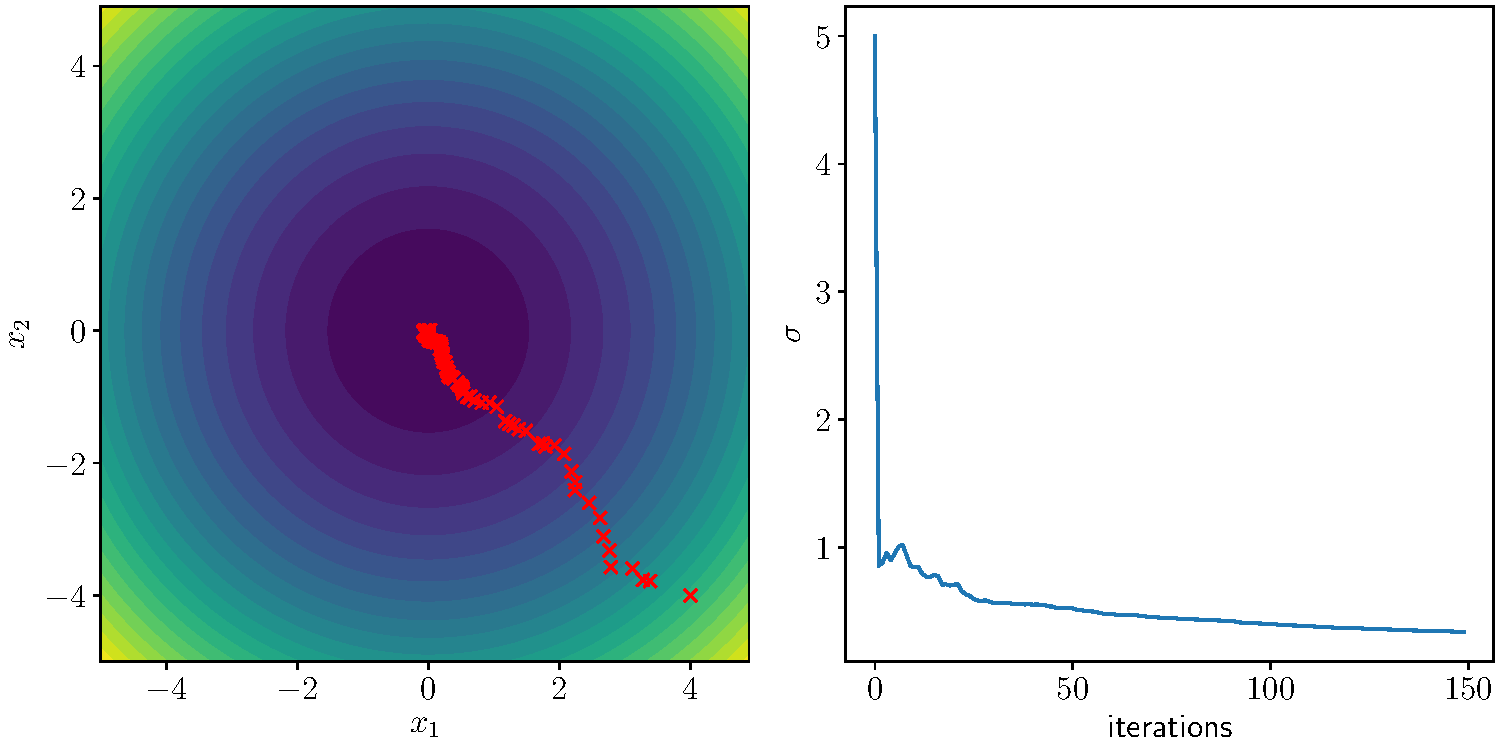
\includegraphics[width=\linewidth]{../figures/TUM/theta_evolution_VO_2023_02_21-03_34_28_PM.pdf}
		\caption{}
		\label{fig:VO_no_cons}
	\end{subfigure}
	\begin{subfigure}{0.75\textwidth}
		\centering
		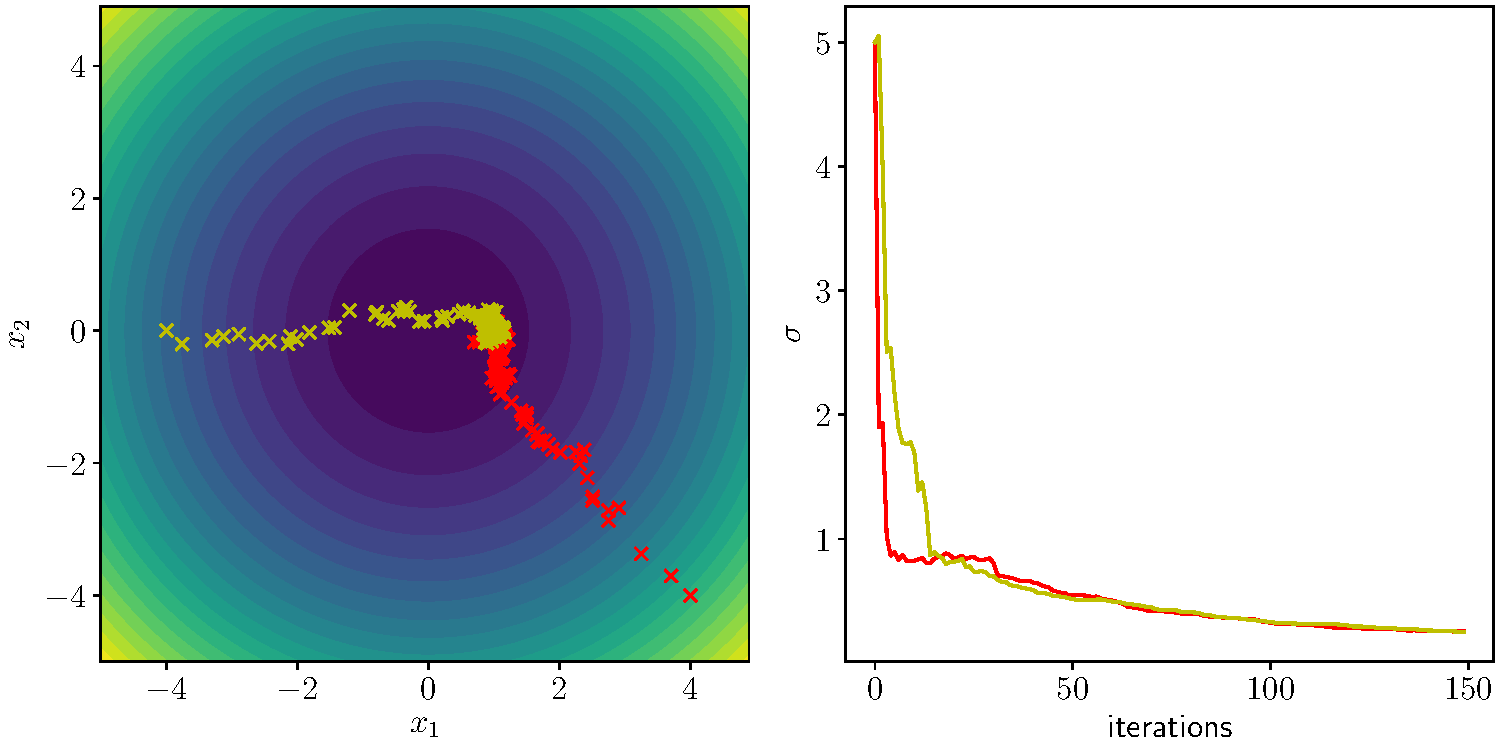
\includegraphics[width=\linewidth]{../figures/TUM/theta_evolution_VO_constraints_2023_02_24-05_12_07_PM.pdf}
		\caption{}
		\label{fig:VO_constraints}
	\end{subfigure}
	\caption{\emph{Stochastic VO for constrained and unconstrained quadratic function}: (a) This is for case when constraints are not present. The left plot shows how the Gaussian mean $\mu$ move towards the minimum of objective despite noisy gradients, the right plots the learned $\sigma$ values versus the gradient descent iterations (b) This is for a constraint on $\bm{x} (x_1 \geq 1)$. The left plot shows how the Gaussian mean $\mu$ moves towards the optimum (for two different starting values) while trying to satisfy the constraint and the right plots the learned $\sigma$ values versus the gradient descent iterations   }
	\label{fig:VO}
\end{figure}

\begin{mdframed}
	\textbf{Open research question/Novelty :} 
	\begin{enumerate}
		\item Why not use finite differences to approximate gradients?: With the constraints, the augmented objective is $C^0$, so the gradients are not even defined at that point.
		\item Then why not use Bayesian Optimization? \atul{Bayesian optimization is difficult for $(dim \geq 10)$. Also constraints are "difficult" in Bayesian optimization. The VO most probably will also struggle in high dimention. Have to check. But including constraints is not that difficult. Stelios: For the current toy problem, BO may be better (because objective has no random variable). But for the problem when the objective has implicit dependance on the design variable (through a random variable), BO makes no sense. The objective would not be known}
		\item To test in high dimention, Will it make sense to test the VO with the following?:
		\begin{align}
			f(x) = \frac{1}{200}\sum_{i=1}^{100} x_i^2 \quad \text{s.t} \quad x_i\geq1
		\end{align}
		The $\bm{x}^*$ would be a unit vector.
	\end{enumerate}
\end{mdframed}


\subsection{Performance based concrete design}

\begin{figure}[!htpb]
	\centering
	\begin{tikzpicture}
		\node (theta) at (-1,-2) {$\theta$};
		\node (x_1) at (0,0) {$x_1$};
		\node (x_2) at (0,-2) [circle, draw, dotted] {$x_2$};
		\node (b_1) at (1,1) [circle, draw] {$\bm{b}_1$}; % can add fill=black!20
		\node (b_2) at (1,0) [circle, draw] {$\bm{b}_2$};
		\node (y_1) at (3,1) [rectangle, draw] {$y_1$};
		\node (y_2) at (3,0) [rectangle, draw] {$y_2$}; 
		\node (y_3) at (3,-1) [rectangle, draw] {$y_3$}; 
		\node (y_4) at (3,-2) [rectangle, draw] {$y_4$}; 
		\node (C_1) at (5,1) [rectangle, draw] {$\mathcal{C}_1\left(y_1(\cdot)\right)$}; 
		\node (C_2) at (5,0) [rectangle, draw] {$\mathcal{C}_2\left(y_2(\cdot)\right)$}; 
		\node (C_3) at (5,-1) [rectangle, draw] {$\mathcal{C}_3\left(y_3(\cdot)\right)$}; 
		\node (O) at (5,-2) [rectangle, draw] {$\mathcal{O}\left(y_4(\cdot)\right)$}; 
		
		\graph {
			%A [as=$\mathcal{A}$, shape = none, "$P(A)$"];
			%B [as=$B$, shape=rectangle ,"$P(B)$"];
			%C [as=$C$,fill=black!20 , "$P(C|A,B)$"];
			
			(x_1) -> {(b_1),(b_2),(y_4)};
			(b_1) -> {(y_1),(y_2),(y_3)};
			(b_2) -> {(y_1),(y_2),(y_3)};
			(y_1) -> (C_1);
			(y_2) -> (C_2);
			(y_3) -> (C_3);
			(y_4) -> (O);
			(theta) -> (x_2);
			(x_2) -> {(y_1),(y_2),(y_3),(y_4)};
			
		};
	\end{tikzpicture}
	\caption{\emph{Stochastic computational graph for the constraint optimization problem for the performance based concrete design:} The circle represents \textit{stochastic nodes}, rectangle the \textit{deterministic node} and no shape is for the \textit{input nodes} (design variables). The objective and the constraints are explicitly dependant on the design variable $x_2$ and they are not differentiable w.r.t it (Hence $x_2$ in dotted). So based on our discussions above, $x_2 \sim q(x_2\mid\theta)$. Several other deterministic nodes are present between the random variables $\bm{b}_1$,$\bm{b}_2$ and the KPIs $y_1, y_2, y_3, y_4$ but they are ignored for brevity.}
	\label{fig:stochastic graph demonstrator}
\end{figure}

The interconnected graph in Figure. \ref{label} can be represented in term of probabilistic graphs as discussed in Figure. \ref{fig:stochastic graph demonstrator}

\atul{This section will involve the calibration results and then the optimization results. The concrete model discussed in section 2 IMO should be in a form accessible to computational science community, with details elaborated in Appendix. Drawing from discussions in section 2, we can discuss the results here.}


\section{Example code from template}

Tables can be inserted via the normal table and tabular environment. 
\begin{table}[h]
\begin{center}
\begin{minipage}{174pt}
\caption{Caption text}\label{tab1}%
\begin{tabular}{@{}llll@{}}
\toprule
Column 1 & Column 2  & Column 3 & Column 4\\
\midrule
row 1    & data 1   & data 2  & data 3  \\
row 2    & data 4   & data 5\footnotemark[1]  & data 6  \\
row 3    & data 7   & data 8  & data 9\footnotemark[2]  \\
\botrule
\end{tabular}
\footnotetext{Source: This is an example of table footnote. This is an example of table footnote.}
\footnotetext[1]{Example for a first table footnote. This is an example of table footnote.}
\footnotetext[2]{Example for a second table footnote. This is an example of table footnote.}
\end{minipage}
\end{center}
\end{table}

\noindent

\begin{table}[h]
\begin{center}
\begin{minipage}{\textwidth}
\caption{Example of a lengthy table which is set to full textwidth}\label{tab2}
\begin{tabular*}{\textwidth}{@{\extracolsep{\fill}}lcccccc@{\extracolsep{\fill}}}
\toprule%
& \multicolumn{3}{@{}c@{}}{Element 1\footnotemark[1]} & \multicolumn{3}{@{}c@{}}{Element 2\footnotemark[2]} \\\cmidrule{2-4}\cmidrule{5-7}%
Project & Energy & $\sigma_{calc}$ & $\sigma_{expt}$ & Energy & $\sigma_{calc}$ & $\sigma_{expt}$ \\
\midrule
Element 3  & 990 A & 1168 & $1547\pm12$ & 780 A & 1166 & $1239\pm100$\\
Element 4  & 500 A & 961  & $922\pm10$  & 900 A & 1268 & $1092\pm40$\\
\botrule
\end{tabular*}
\footnotetext{Note: This is an example of table footnote. This is an example of table footnote this is an example of table footnote this is an example of~table footnote this is an example of table footnote.}
\footnotetext[1]{Example for a first table footnote.}
\footnotetext[2]{Example for a second table footnote.}
\end{minipage}
\end{center}
\end{table}

In case of double column layout, tables which do not fit in single column width should be set to full text width. For this, you need to use \verb+\begin{table*}+ \verb+...+ \verb+\end{table*}+ instead of \verb+\begin{table}+ \verb+...+ \verb+\end{table}+ environment. Lengthy tables which do not fit in textwidth should be set as rotated table. For this, you need to use \verb+\begin{sidewaystable}+ \verb+...+ \verb+\end{sidewaystable}+ instead of \verb+\begin{table*}+ \verb+...+ \verb+\end{table*}+ environment. This environment puts tables rotated to single column width. For tables rotated to double column width, use \verb+\begin{sidewaystable*}+ \verb+...+ \verb+\end{sidewaystable*}+.

\begin{sidewaystable}
\sidewaystablefn%
\begin{center}
\begin{minipage}{\textheight}
\caption{Tables which are too long to fit, should be written using the ``sidewaystable'' environment as shown here}\label{tab3}
\begin{tabular*}{\textheight}{@{\extracolsep{\fill}}lcccccc@{\extracolsep{\fill}}}
\toprule%
& \multicolumn{3}{@{}c@{}}{Element 1\footnotemark[1]}& \multicolumn{3}{@{}c@{}}{Element\footnotemark[2]} \\\cmidrule{2-4}\cmidrule{5-7}%
Projectile & Energy	& $\sigma_{calc}$ & $\sigma_{expt}$ & Energy & $\sigma_{calc}$ & $\sigma_{expt}$ \\
\midrule
Element 3 & 990 A & 1168 & $1547\pm12$ & 780 A & 1166 & $1239\pm100$ \\
Element 4 & 500 A & 961  & $922\pm10$  & 900 A & 1268 & $1092\pm40$ \\
Element 5 & 990 A & 1168 & $1547\pm12$ & 780 A & 1166 & $1239\pm100$ \\
Element 6 & 500 A & 961  & $922\pm10$  & 900 A & 1268 & $1092\pm40$ \\
\botrule
\end{tabular*}
\footnotetext{Note: This is an example of table footnote this is an example of table footnote this is an example of table footnote this is an example of~table footnote this is an example of table footnote.}
\footnotetext[1]{This is an example of table footnote.}
\end{minipage}
\end{center}
\end{sidewaystable}



% supplementary information, acknowledgements, declarations, etc

\backmatter

\bmhead{Supplementary information}

If your article has accompanying supplementary file/s please state so here. 

Authors reporting data from electrophoretic gels and blots should supply the full unprocessed scans for key as part of their Supplementary information. This may be requested by the editorial team/s if it is missing.

Please refer to Journal-level guidance for any specific requirements.

\bmhead{Acknowledgments}

Acknowledgments are not compulsory. Where included they should be brief. Grant or contribution numbers may be acknowledged.

Please refer to Journal-level guidance for any specific requirements.

\section*{Declarations}

Some journals require declarations to be submitted in a standardised format. Please check the Instructions for Authors of the journal to which you are submitting to see if you need to complete this section. If yes, your manuscript must contain the following sections under the heading `Declarations':

\begin{itemize}
\item Funding
\item Conflict of interest/Competing interests (check journal-specific guidelines for which heading to use)
\item Ethics approval 
\item Consent to participate
\item Consent for publication
\item Availability of data and materials
\item Code availability 
\item Authors' contributions
\end{itemize}

\noindent
If any of the sections are not relevant to your manuscript, please include the heading and write `Not applicable' for that section. 

%%===================================================%%
%% For presentation purpose, we have included        %%
%% \bigskip command. please ignore this.             %%
%%===================================================%%
\bigskip
\begin{flushleft}%
Editorial Policies for:

\bigskip\noindent
Springer journals and proceedings: \url{https://www.springer.com/gp/editorial-policies}

\bigskip\noindent
Nature Portfolio journals: \url{https://www.nature.com/nature-research/editorial-policies}

\bigskip\noindent
\textit{Scientific Reports}: \url{https://www.nature.com/srep/journal-policies/editorial-policies}

\bigskip\noindent
BMC journals: \url{https://www.biomedcentral.com/getpublished/editorial-policies}
\end{flushleft}


\begin{appendices}
	
\section{Section title of first appendix}\label{secA1}
An appendix contains supplementary information that is not an essential part of the text itself but which may be helpful in providing a more comprehensive understanding of the research problem or it is information that is too cumbersome to be included in the body of the paper.

%%=============================================%%
%% For submissions to Nature Portfolio Journals %%
%% please use the heading ``Extended Data''.   %%
%%=============================================%%


\end{appendices}

%%===========================================================================================%%
%% If you are submitting to one of the Nature Portfolio journals, using the eJP submission   %%
%% system, please include the references within the manuscript file itself. You may do this  %%
%% by copying the reference list from your .bbl file, paste it into the main manuscript .tex %%
%% file, and delete the associated \verb+\bibliography+ commands.                            %%
%%===========================================================================================%%

\bibliography{optimization_paper_bibliography}% common bib file
%% if required, the content of .bbl file can be included here once bbl is generated
%%\input sn-article.bbl

%% Default %%
%%\input sn-sample-bib.tex%

\end{document}
